\chapter{Implementation of your Project}
\label{ch:Implementation}

\section{Design}
This section presents the design and the key design decisions we made for this project.
We begin by describing the hardware apparatus, which includes the actuators and the gloves themselves, as well as the design iterations undertaken during the development of the glove.
Next, we outline the software components, detailing the encoding of the actuators, the communication protocol, and providing a brief introduction to the associated software elements.
Finally, we conclude this section by introducing the study design of the two studies conducted to address our research questions.


\subsection{Hardware}
We have divided this subsection into two parts: the first focuses on the actuators used, while the second discusses the design of the Velcro gloves.

\subsubsection{Actuator Design}
For the actuators and their setup, we adopted the design and configuration proposed by Fang et al. \cite{Fang2023}, using Velcro straps. This decision was informed by prior research \cite{Markow2010, Kohlsdorf2010, Huang2010, Fang2023a}, which highlights the importance of design factors such as weight, breathability, flexibility, and coarseness for user comfort, particularly during extended wear. Velcro straps effectively meet these criteria while enhancing dexterity, a recognized advantage of fingerless glove designs \cite{Huang2008}. This design facilitates everyday tasks and accommodates a range of finger sizes, making the gloves adaptable for different users. Furthermore, using the same actuators enables a direct comparison with Fang et al.’s prior work \cite{Fang2023}, which employed identical actuators in a one-handed, non-chorded piano learning setup.

The actuators consist of six vibration systems (three per hand), with one shown in \autoref{fig:fang-vibration}. Each system includes a vibration motor (Brand: Grove Seed; Model: ANDA-B1020) housed in a 3D-printed PLA case and secured with Velcro bands. Operating at a frequency of approximately 200 Hz, the vibration motors are directly connected to the glove for control. Each system is mounted in a curved-bottom 3D-printed case for optimal fit, as illustrated in \autoref{fig:fang-vibration}, where it is demonstrated on a single finger. Consistent with Fang et al.’s design \cite{Fang2023}, larger contact areas were used to allow easier adjustment for individual comfort. The actuators operate at an amplitude of 1.03 G and weigh 6.6 grams each.

\begin{figure}
     \centering
     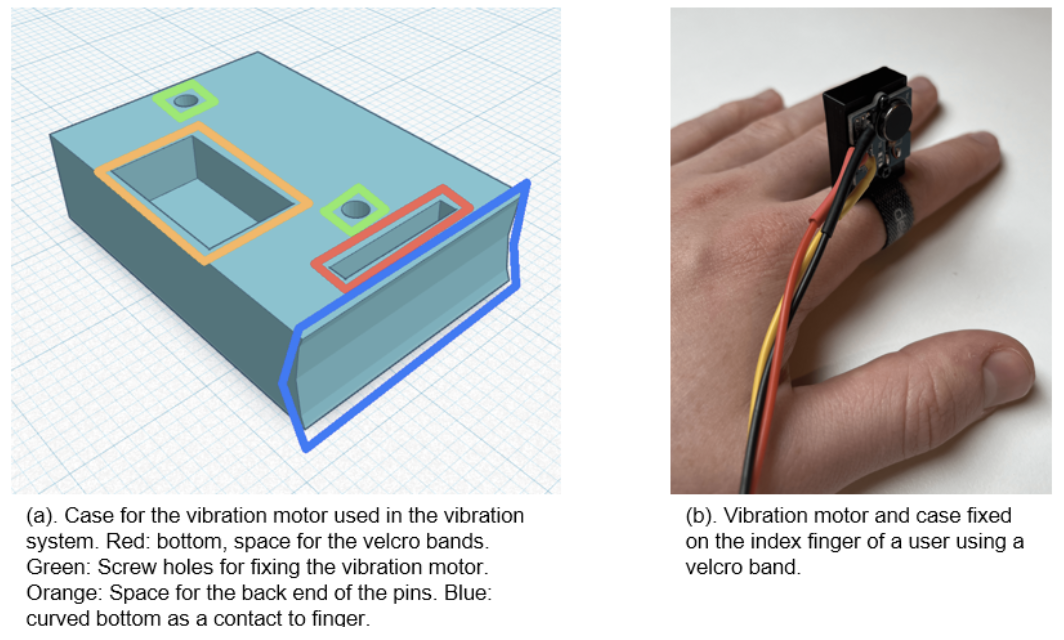
\includegraphics[width=0.5\linewidth]{src/pictures/Screenshot 2024-09-12 at 15.11.57.png}
     \caption{3D model, and the implementation on a users finger of one element of the vibration system from \cite{Fang2023}}
     \label{fig:fang-vibration}
 \end{figure}
\begin{figure}
    \centering
    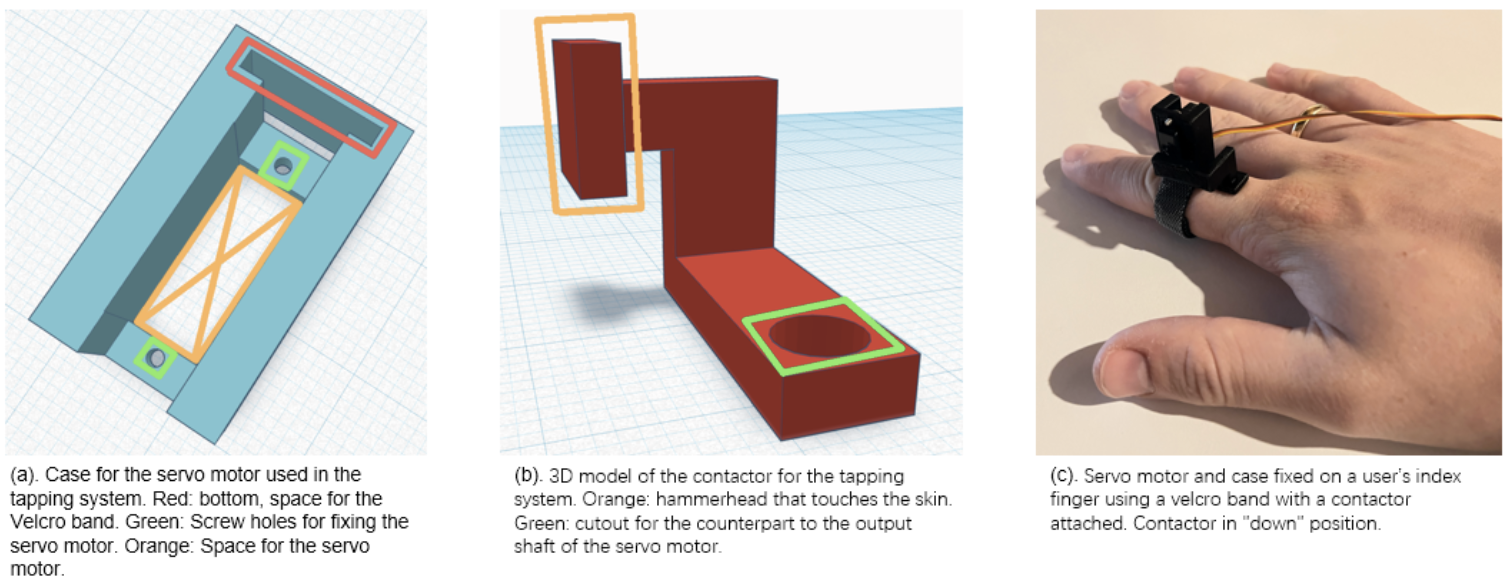
\includegraphics[width=0.5\linewidth]{src/pictures/Screenshot 2024-09-12 at 15.11.38.png}
    \caption{3D models for the case and hammer-shaped contactor, and the implementation on a user’s finger of one element of the tapping system from \cite{Fang2023}}
    \label{fig:fang-tapping}
\end{figure}
\begin{figure}
    \centering
    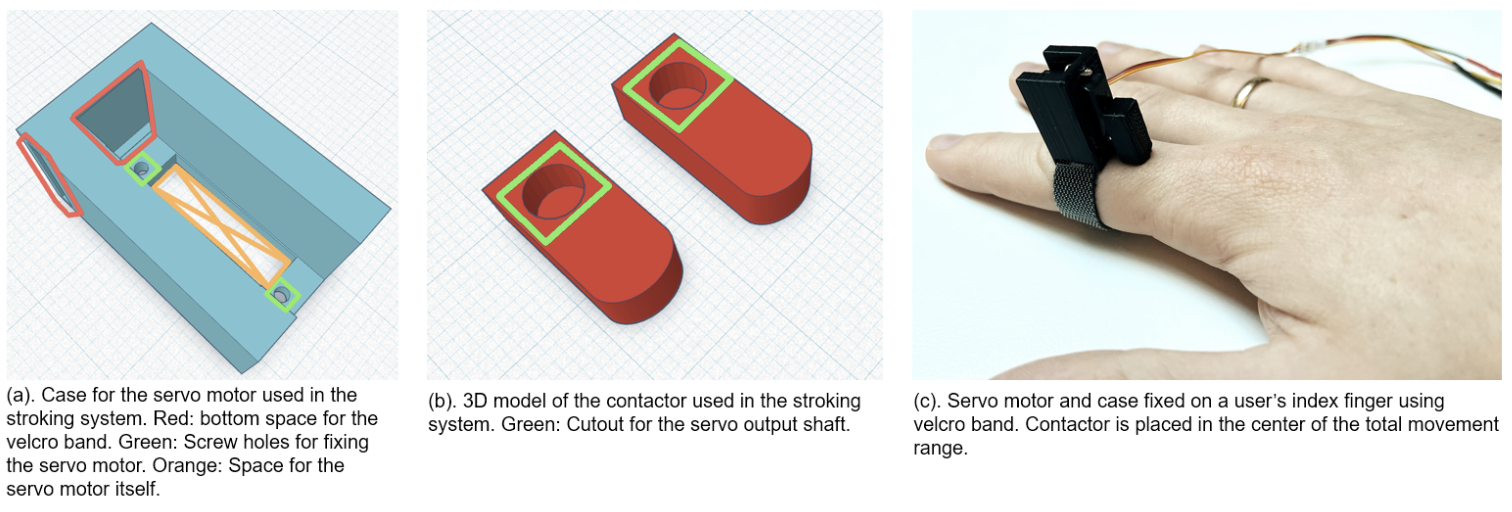
\includegraphics[width=0.5\linewidth]{src/pictures/Screenshot 2024-09-12 at 15.10.49.png}
    \caption{3D models for the case and the contactor, and the implementation on a users finger of one element of the stroking system from \cite{Fang2023}.}
    \label{fig:fang-stroking}
\end{figure}

For the tapping and stroking systems, we employed six actuators for each system, utilizing mini-servo motors (Master DS208). These motors provide an actuating force of approximately 0.1–0.2 kg and complete a 45° movement in approximately 0.1 seconds. The actuators draw around 5V and 1.75A for stroking, and 5V and 2A for tapping, based on our measurements using a 
USB Current Voltage Capacity Tester (Model: KWS-V20/V21).
Both systems are controlled via \gls{pdm} through the glove. The cases for these systems are 3D-printed using PLA. The design of the stroking system is shown in \autoref{fig:fang-stroking}, while the tapping system is depicted in \autoref{fig:fang-tapping}.

To enhance wearer comfort during prolonged use, we added a small cushion to the actuator casings for both the tapping and stroking systems. This cushion, which was not included in Fang et al.’s original design \cite{Fang2023}, and is only used for the contact area of the non-moving part of the actuator and the skin.

The tapping system delivers equal force at the same rate by applying and removing contact from the user’s skin \cite{Fang2023}. Its design follows a hammer-like structure, consisting of a servo motor housed in a PLA case and a contactor. The contactor is an 8 × 8 mm square plate that presses against the skin, connected to the servo motor’s output shaft via an L-shaped support. The design is illustrated in \autoref{fig:fang-tapping}.

The stroking system, shown in \autoref{fig:fang-stroking}, features a contactor that moves across the user’s skin while simultaneously indenting it slightly, similar to the tapping system. The contactor is a 15 × 7 × 5 mm square with a rounded bottom and is housed in a design similar to the tapping system. The servo motor is mounted on the participant’s hand, and by rotating the motor, the contactor performs a stroking motion across the skin.

All actuators are positioned near the interphalangeal joints of the fingers.











\subsubsection{Glove Design and Design Iterations}
\label{Glove_Design_Iteration}
\begin{figure}
    \centering
    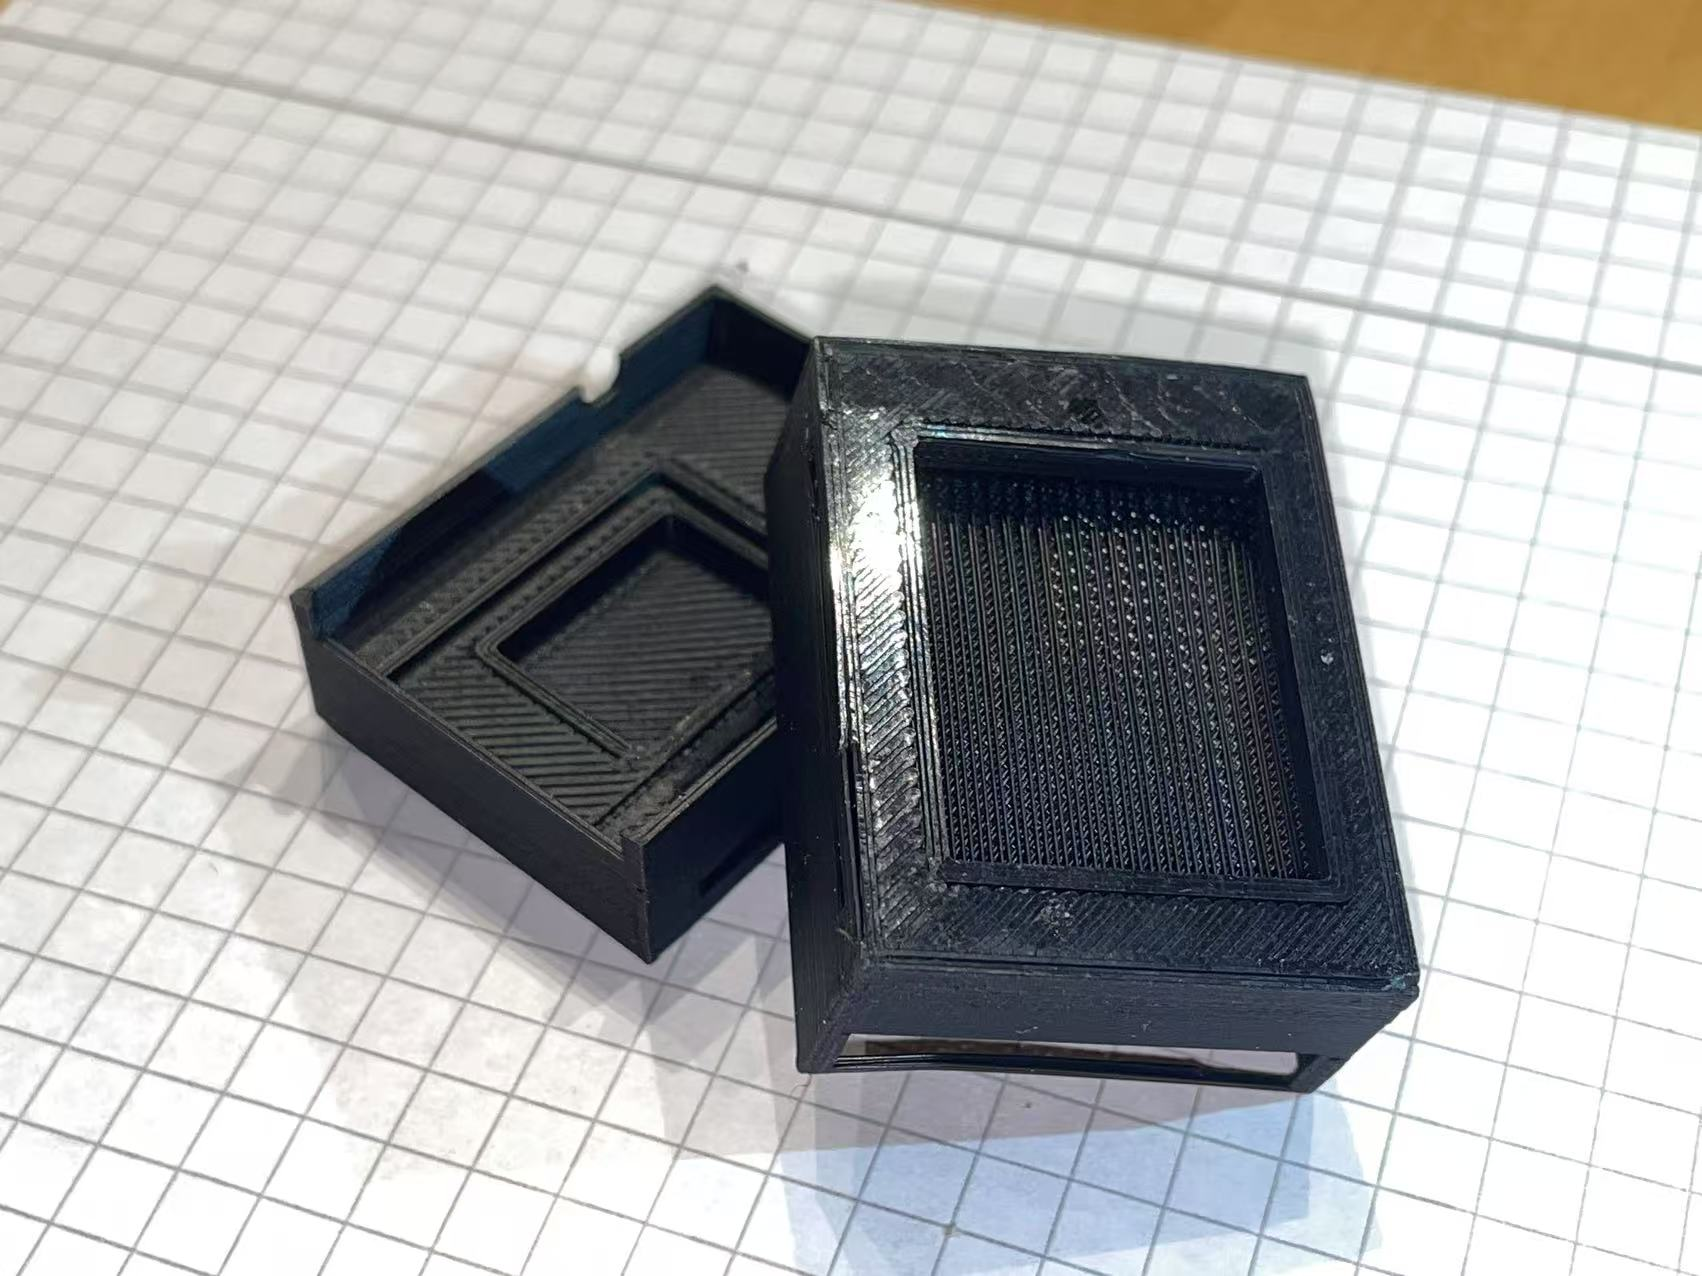
\includegraphics[width=0.5\linewidth]{src/pictures/GloveDesigns/cases.jpg}
    \caption{Final Glove- Case Design on a squared Din A5 paper for size reference.}
    \label{fig:cases}
\end{figure}

\begin{figure}
    \centering
    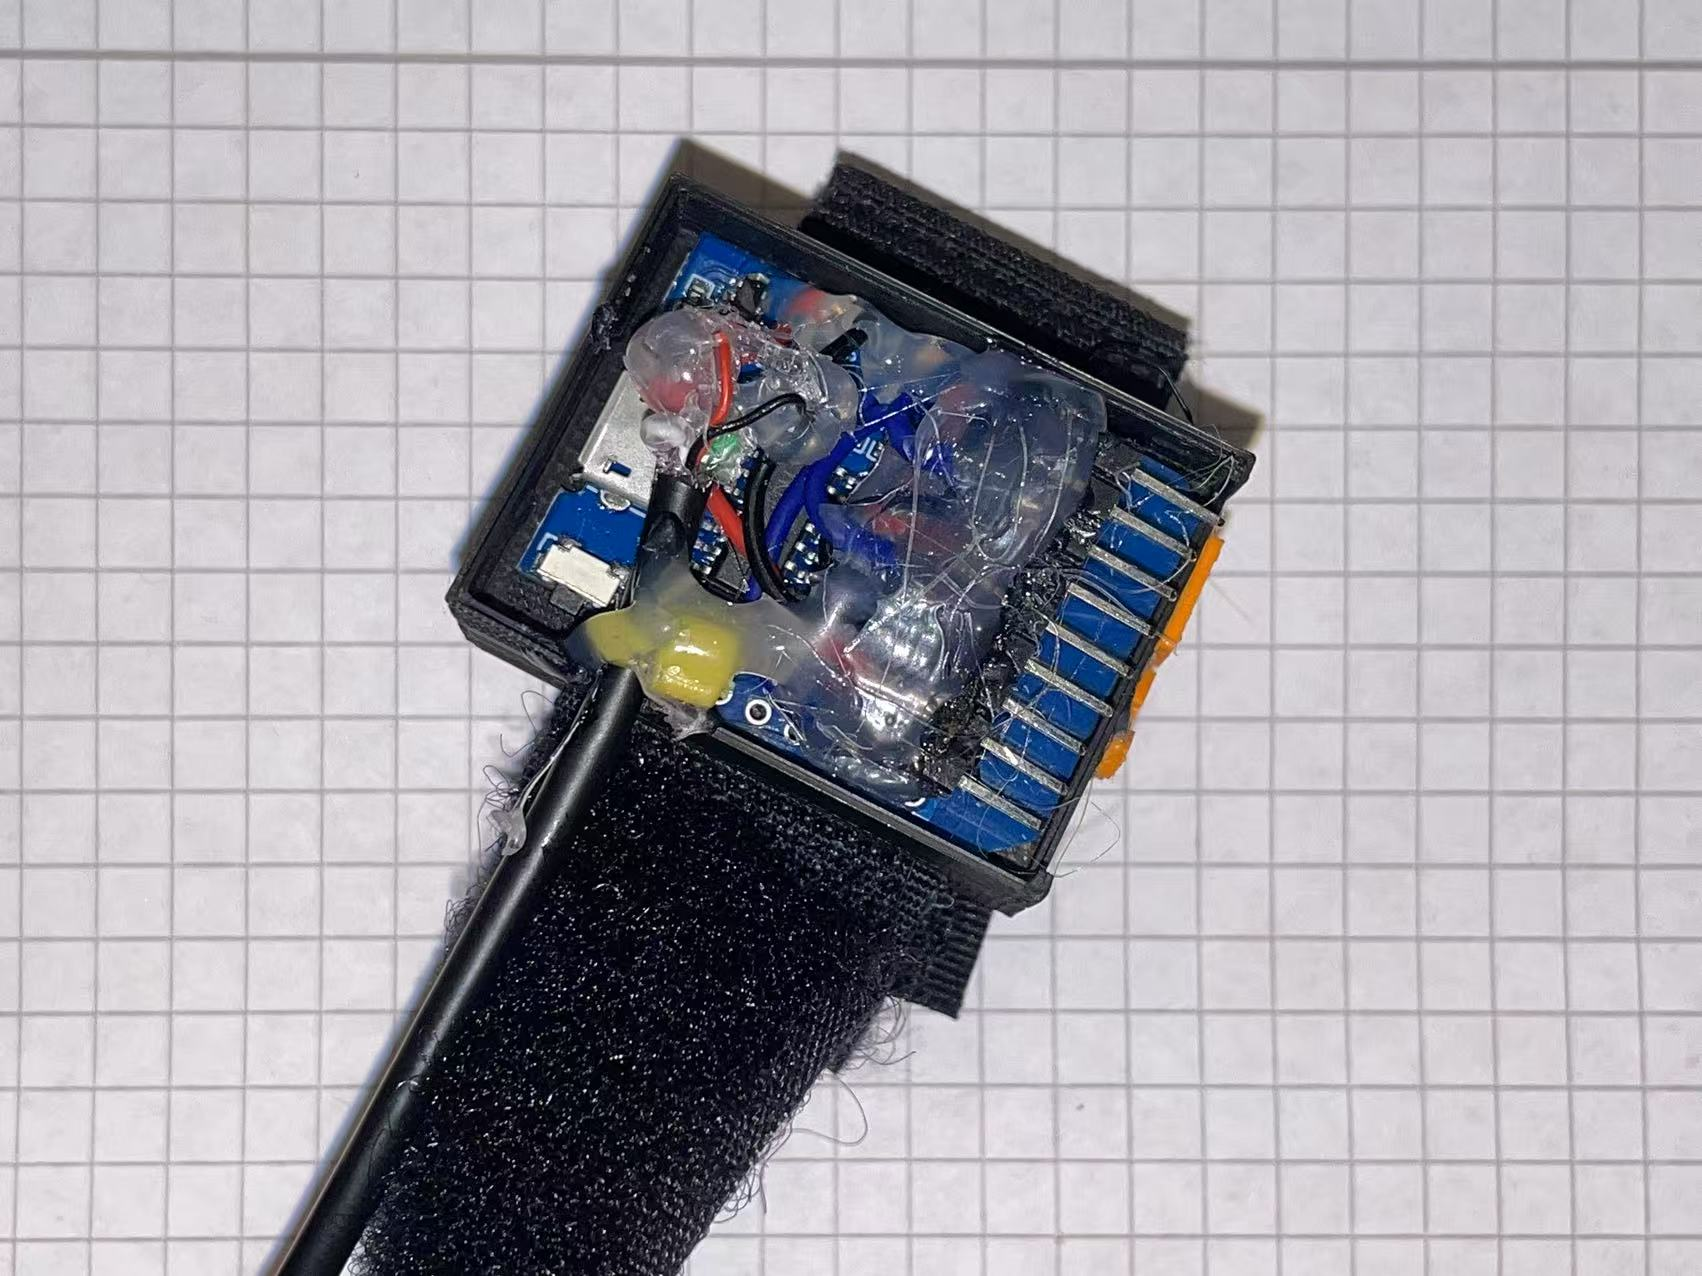
\includegraphics[width=0.5\linewidth]{src/pictures/GloveDesigns/openCase.jpg}
    \caption{Final Glove Design opened on a squared Din A5 paper for size reference.}
    \label{fig:openCases}
\end{figure}

Our final glove design, shown in \autoref{fig:final-glove-design}, incorporates the actuators described above along with a wristband. The wristband consists of a Velcro strap mounted onto a 3D-printed PLA casing with a cushion on the bottom to enhance comfort during extended wear. Herefore, we left a small hole in the bottom to fit the cusion into it due to the cushion being not soft enough due to the clue if not placed within a small indentation as showed in \autoref{fig:cases}.

The casing measures 37.6 mm × 28.75 mm × 15 mm, making it comparable in size to the Xiaomi Mi Watch Lite smartwatch (dimensions: 41 mm × 35 mm × 10.9 mm, weight: 35 g with strap, 21 g without strap)\footnote{\url{https://www.mi.com/de/mi-watch-lite/specs/}}. Also the bottom is fitted, so that the ESP8266 can fit even without glue in there and won't move.
With a open case the design is depicted here \autoref{fig:openCases}. The 9 outputs are the same as depicted in the circuit diagram in \autoref{fig:circuit-diagram}.

This design achieves our goal of creating a compact wearable device comparable to a modern smartwatch.



\begin{figure}
    \centering
    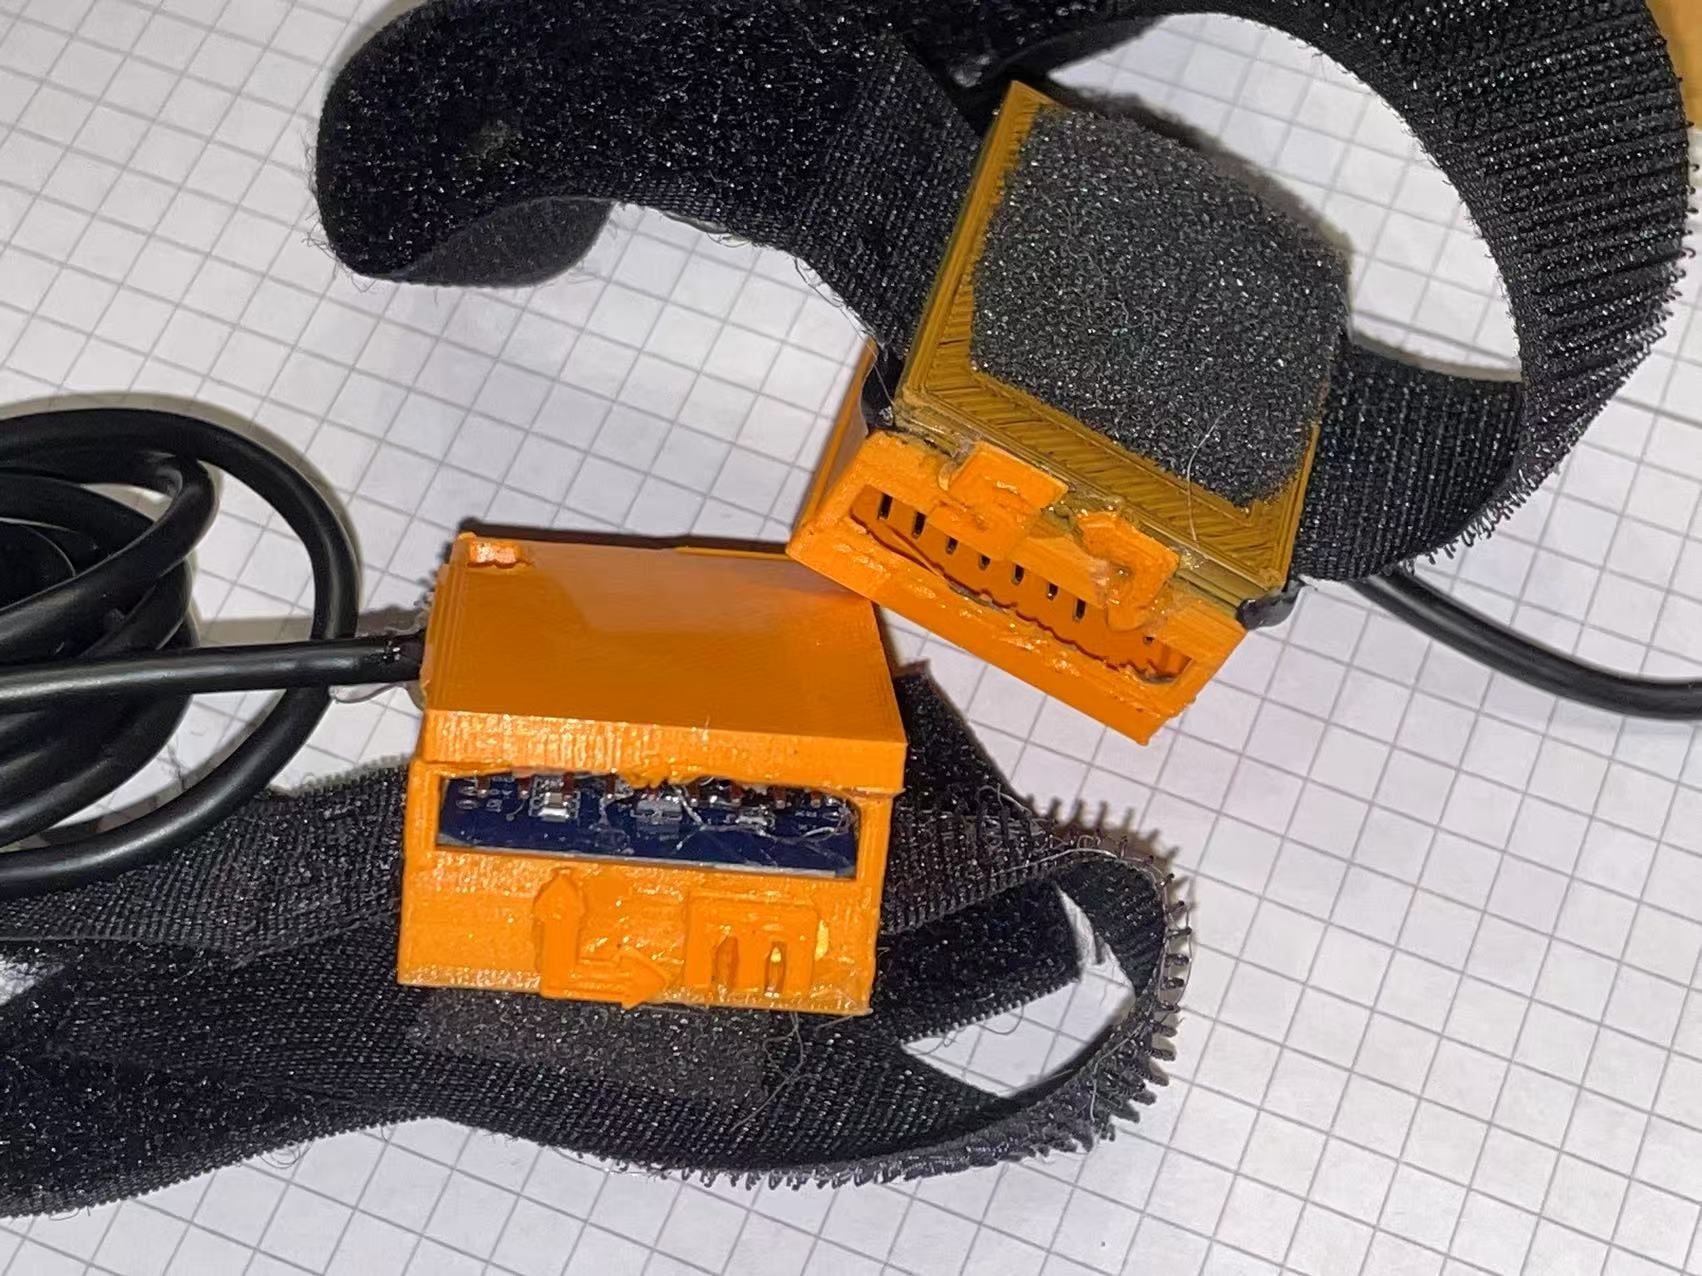
\includegraphics[width=0.5\linewidth]{src/pictures/GloveDesigns/casesFinished.jpg}
    \caption{Final Glove Design on a squared Din A5 paper for size reference.}
    \label{fig:final-glove-design}
\end{figure}


\begin{table}
    \centering
    \resizebox{\columnwidth}{!}{
    \begin{tabular}{cccccccc}
        \textbf{Protocoll}   & \textbf{Range} & \textbf{EE (R)} & \textbf{EE (T)} & \textbf{Throughput} & \textbf{Latency} & \textbf{Overhead} & \textbf{OSI-Layer}\\
        \textbf{ESP-NOW}     & 220m & 489 mW & 1042 mW           & \textbf{1 Mbps} & \textbf{~1ms} & \textbf{Small} & Layer 2\\
        \textbf{TCP / UDP}         & 100m & 214 mW & 538 mW & \textbf{54 Mbps} & ~3.3ms & Medium & Layer 4\\
        \textbf{Bluetooth}   & 60m & 141 mW & 441 mW       & ~784 Kbps & ~6ms & High & Layer 2\\
    \end{tabular}}
    \caption{Comparison of Wi-Fi, Bluetooth and Esp-Now \cite{eridani2021comparative}.\\EE stands for Energy Efficiency, R stands for receiver and T for transmitter.}
    \label{tab:comparissonESPNOW}
\end{table}

For the microcontroller, we chose to use devices from the ESP family due to their compatibility with the ESP-Now protocol. This decision was based on the protocol's advantages in terms of latency, overhead, and throughput, as highlighted in the comparison by Eridani et al. \cite{eridani2021comparative}, with their results shown in \autoref{tab:comparissonESPNOW}. As we identified those as the most important criteria for solving our  soft-real time\footnote{Soft-Real Time as defined in computational theory such as by Shin et al. \cite{shin1994real}} requirements, as we need to get the ms timings right and in order.

\begin{figure}
    \centering
    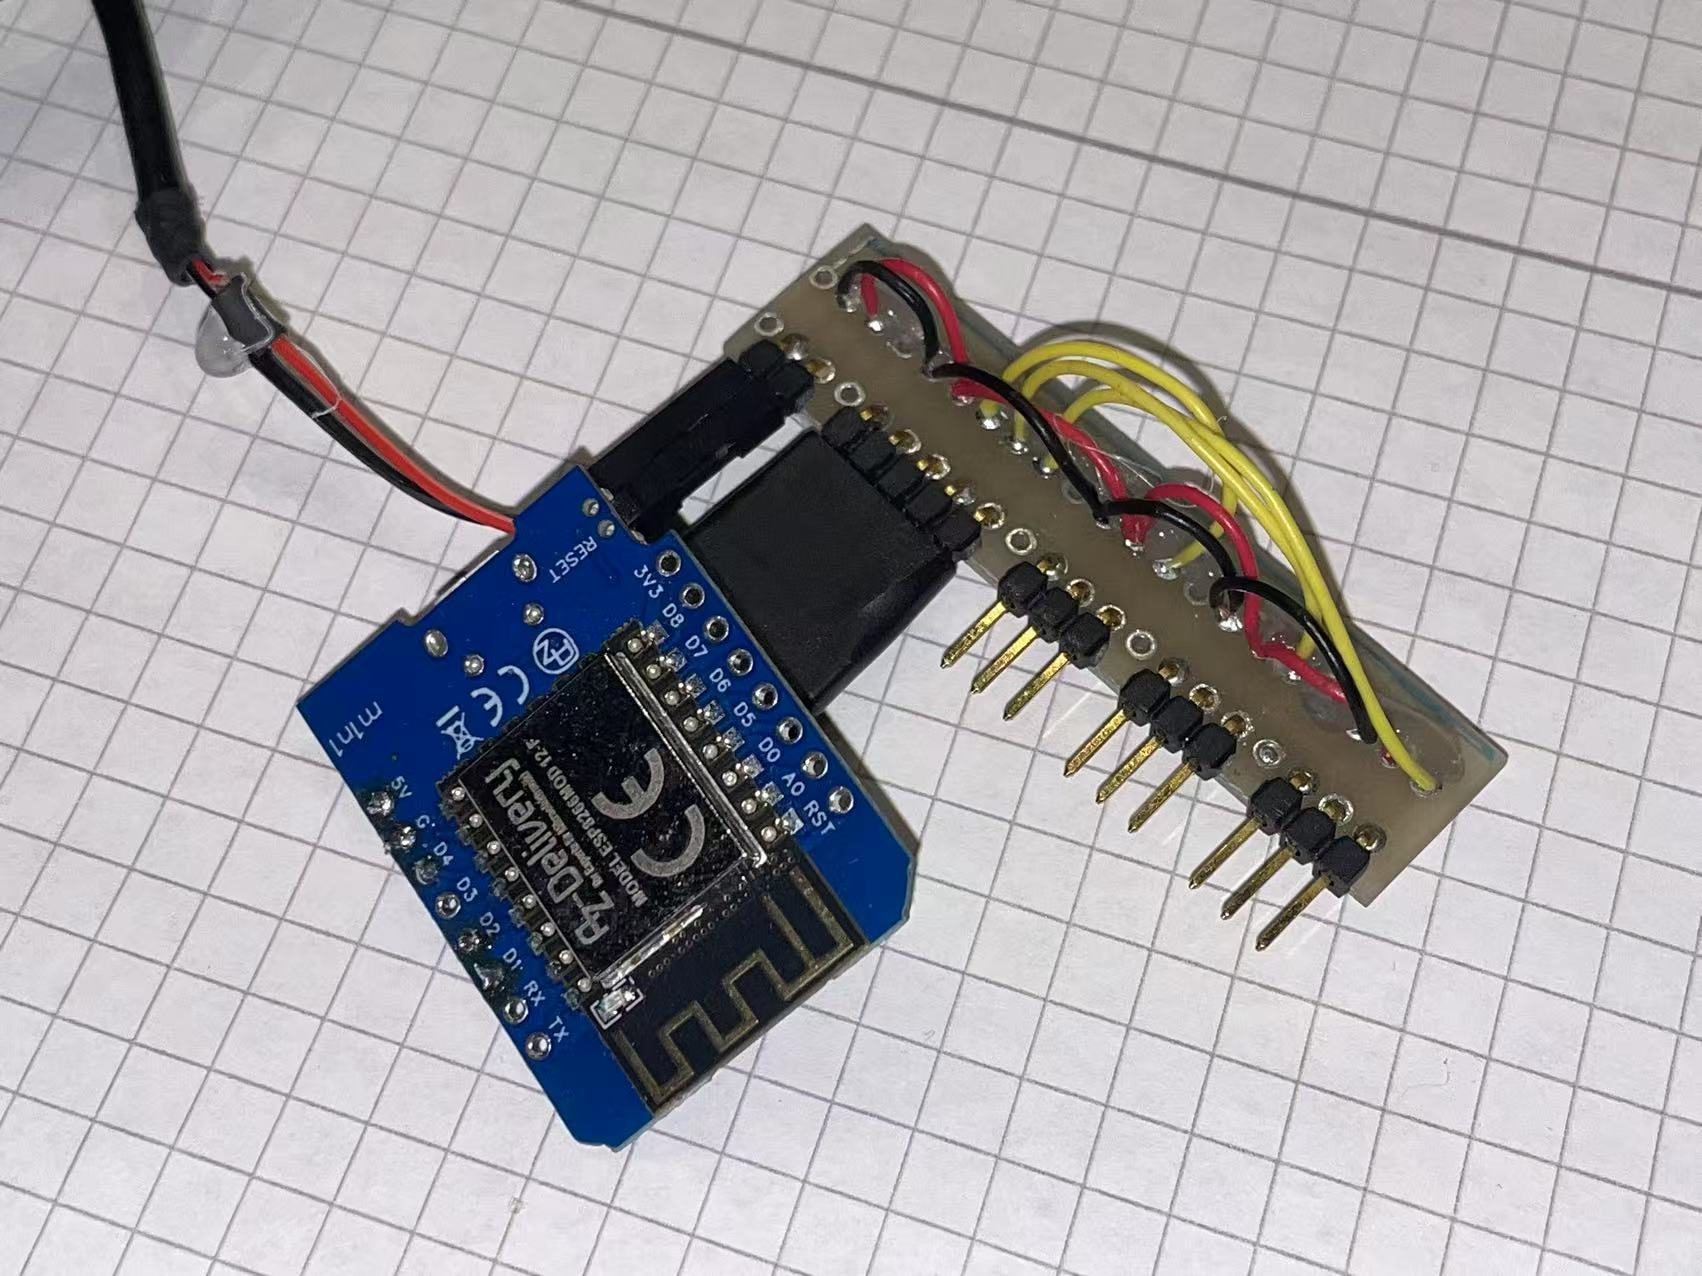
\includegraphics[width=0.5\linewidth]{src/pictures/GloveDesigns/oldDesign.jpg}
    \caption{Old design of the circuit.}
    \label{fig:oldDesign}
\end{figure}

In our initial design iteration, we used the ESP8266 microcontroller, but it was later replaced with the ESP8266 D1 Mini due to several advantages. These include its low cost (approximately €1), lightweight design (3 g)\footnote{\url{https://www.smart-prototyping.com/Mini-D1-PRO-Development-Board-ESP8266-4M-16M}}, and compact size. Both microcontrollers offer built-in Wi-Fi capabilities that provide sufficient connectivity for the entire software system. The affordability and accessibility of the ESP8266 D1 Mini make it particularly suitable for use in low-income households, enhancing the device's feasibility and reach.

The first alpha prototype version with the esp8266 D1 mini is shown in \autoref{fig:oldDesign}. As it is the \gls{mvp}, it is rather bulky with the cables attached to it. Nevertheless, the same circuit diagram as in \autoref{fig:circuit-diagram} applies for it, and it is fully operational.

\begin{figure}
    \centering
    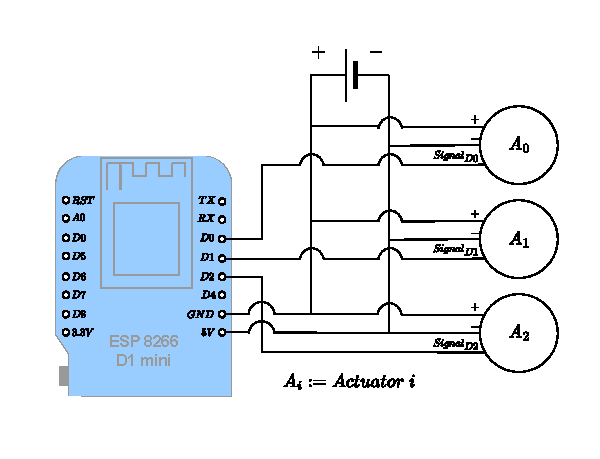
\includegraphics[width=0.5\linewidth]{src/pictures/CircuitDiagramGlove.drawio.pdf}
    \caption{Glove Circuit Diagram.}
    \label{fig:circuit-diagram}
\end{figure}


Due to the high current demands of the tapping and stroking systems, the on-board power supply of the ESP8266 was insufficient. To resolve this, we soldered an additional USB cable to the board to provide an external power supply, as shown in \autoref{fig:circuit-diagram}, that can also be seen on \autoref{fig:oldDesign} for the \gls{mvp} and in \autoref{fig:openCases} for the current one.
In the first experiment, the actuators were interchangeable and could be of the vibration, tapping, or stroking type.
We utilized the pins D0, D1, and D2 because of their \gls{pdm} capabilities.

The USB cable was connected to a standard phone charger. For testing, we used the original 10W Xiaomi USB-A charger (model: MDY-09-EW), which has a maximum output voltage of 5V and 2.0A. This served as the general power source for the system, with one charger used per glove. The design also works with a powerbank, however due to our extended experiment times we didn't use a powerbank in our study.

Furthermore, we added additional wiring to simplify mounting the actuators onto the wristband glove, ensuring better usability and stability during operation.
Which can be seen in the open version of the glove design depicted in \autoref{fig:openCases}, so that we can fit the actuators directly on it.




\subsection{Software}

This software section is divided into two parts, the webistes created for the experiment (one on the glove and one on an external laptop for testing) as well as the communication protocoll used between the gloves.



\subsubsection{Website}
\label{sub:website}
Two websites were developed for the study, adhering to the Material Design guidelines for button design and usability\footnote{\url{https://m3.material.io/}}. One website was displayed on a mobile phone (Xiaomi A2 Lite), which was hosted by the glove to control the experiment and play audio data, while the other was used to assess the participants' knowledge.

The website for controlling speech output and vibrations is shown in \autoref{fig:Website-Design}. It was designed using a responsive framework, enabling compatibility with other devices capable of running modern browsers. During the study, we used the Google Chrome browser on the smartphone.

The website could be accessed within the "Master Glove" Wi-Fi network (SSID: Master Glove) using the URL \url{192.168.4.1}.
The preset buttons on the website correspond to those used in the studies.
Upon pressing a button, the master controller receives the associated word or letter, as well as whether \gls{ost}-Encoding is activated (inactive for sequential input).
The master controller then sends this data to the slave controller.

The website plays the corresponding audio for the selected character using a JavaScript text-to-speech converter, as the master controller was not connected to the internet.
After the specified offset detailed in the audio-vibration offset section, the vibration begins, aligned with the encoding chords and tailored to finger sensitivity.
Both, the audio and vibrations automatically stop after five minutes, providing a break for the conductor to test the participant, as outlined in the study protocol.

\begin{figure}
    \centering
    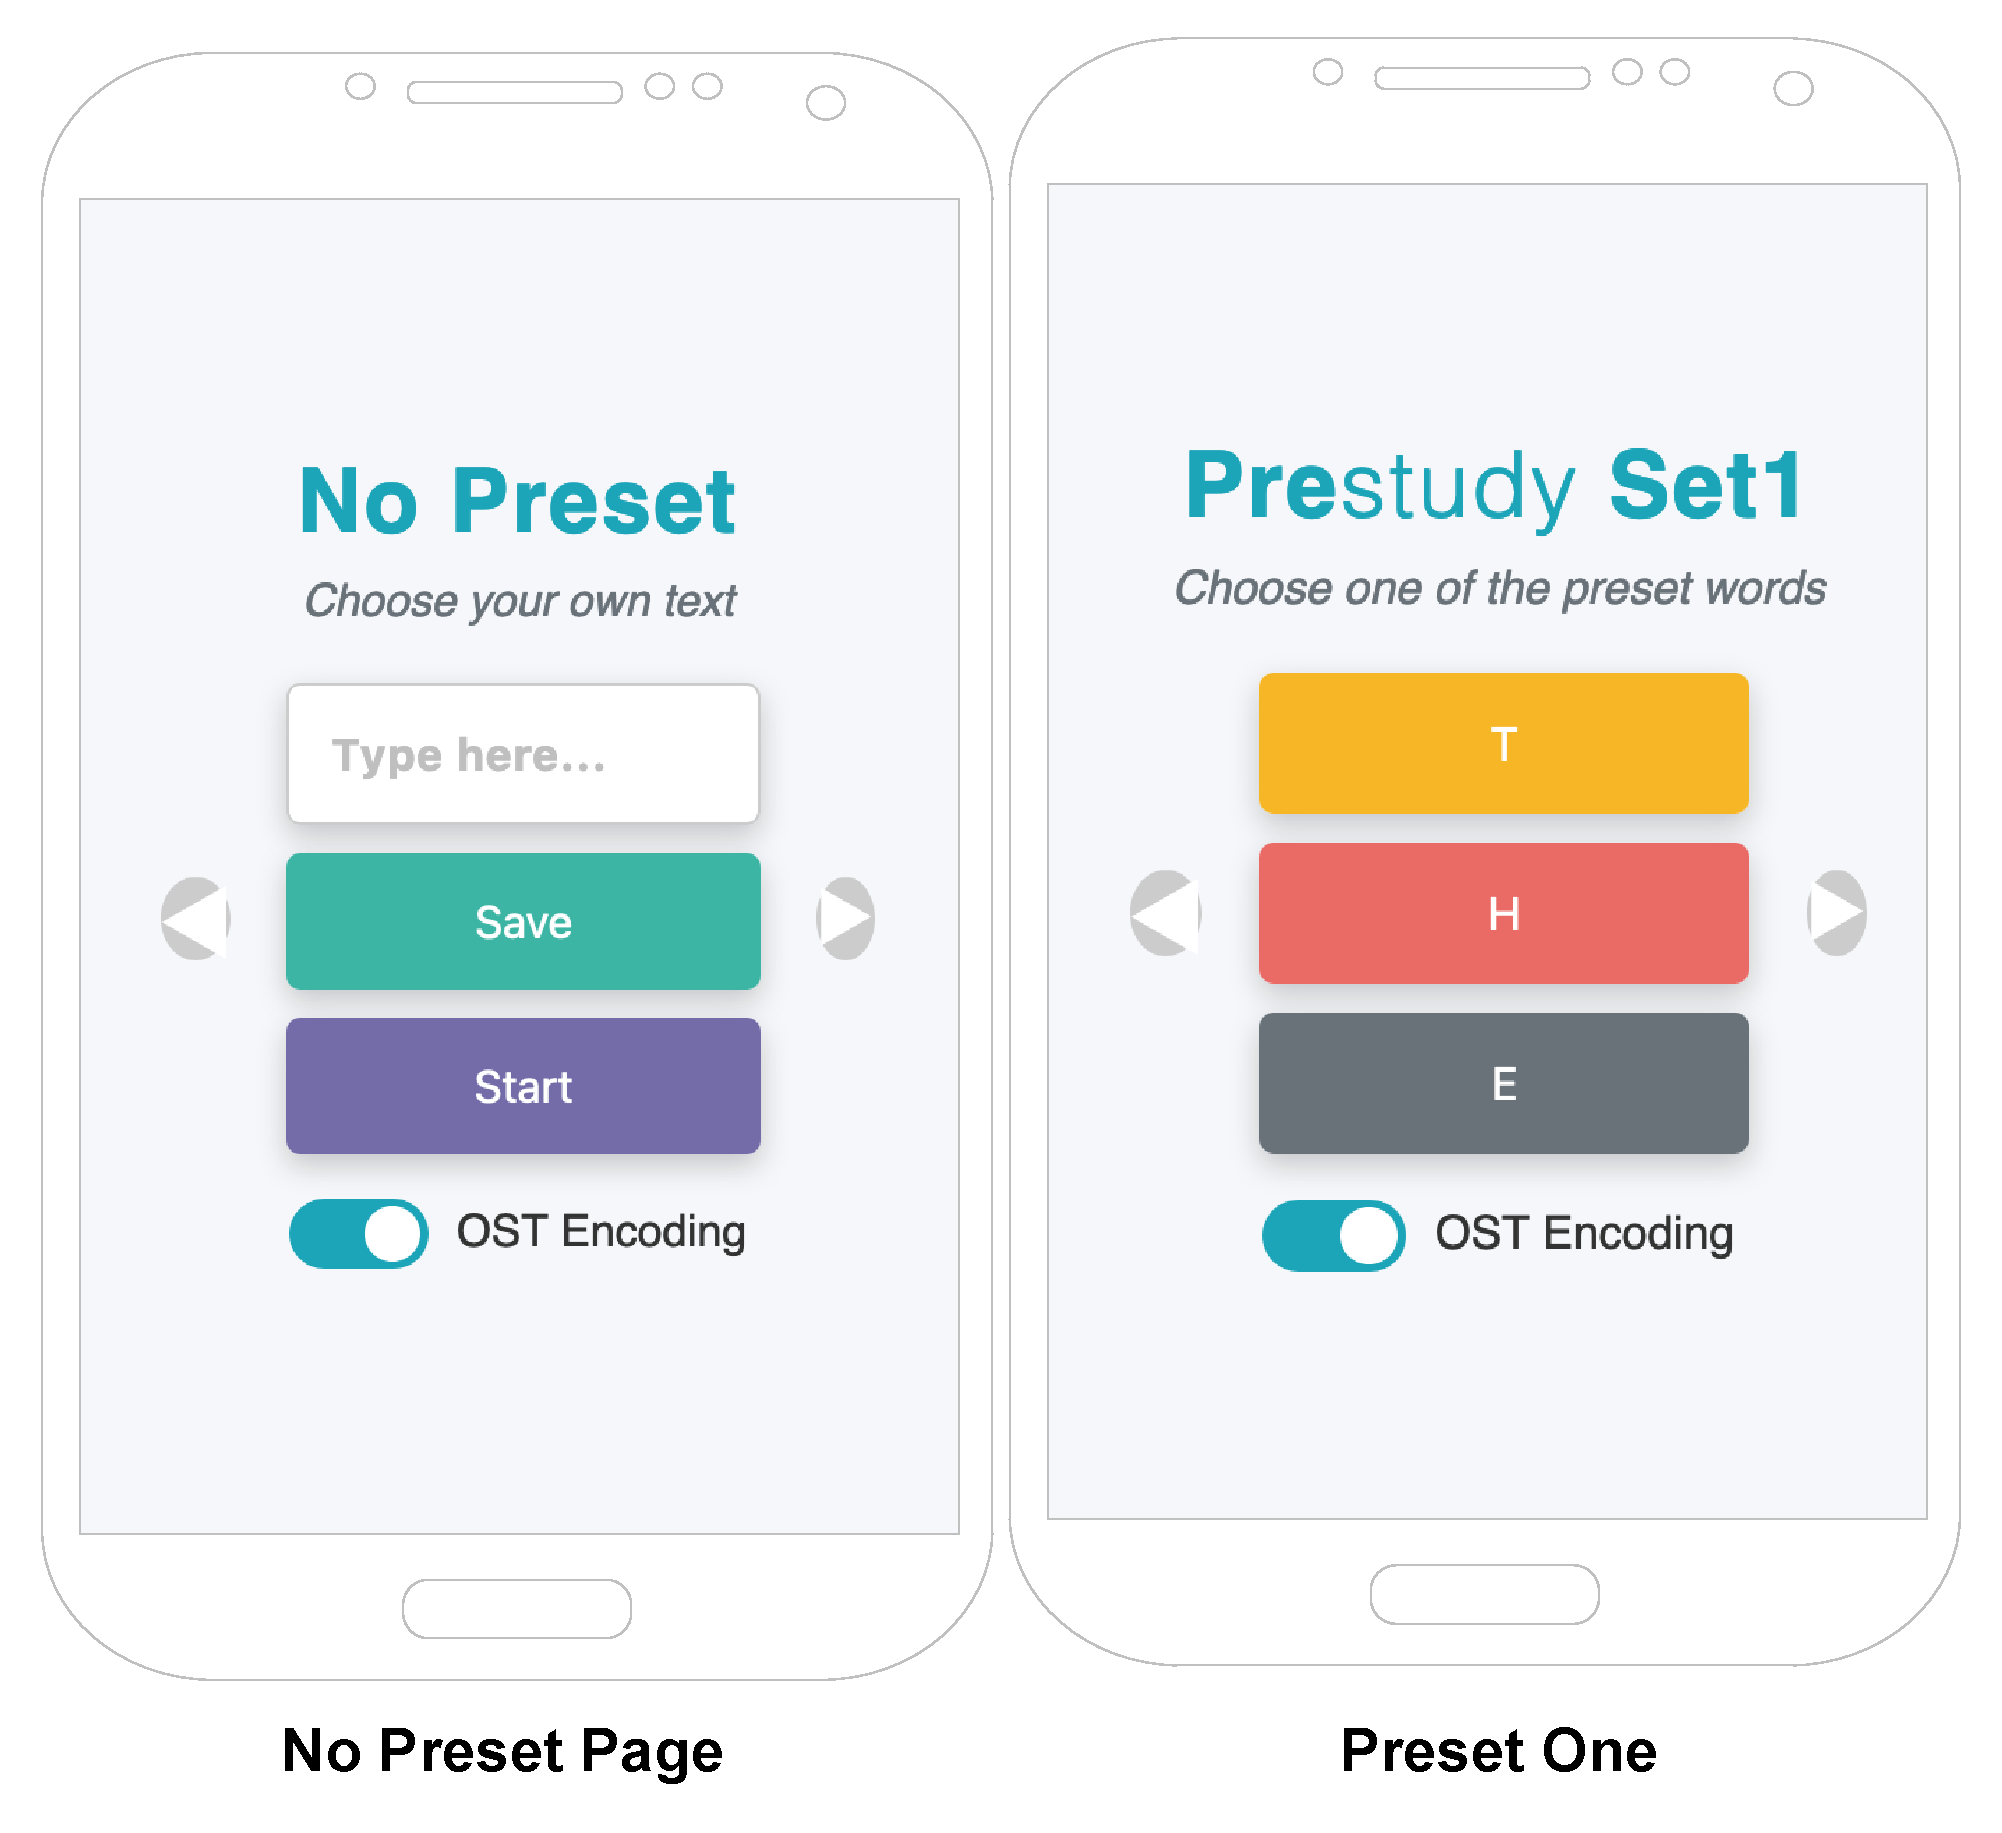
\includegraphics[width=0.5\linewidth]{src/pictures/MobileWebsiteVersion.drawio.pdf}
    \caption{Website Design in a Mobile Phone.}
    \label{fig:Website-Design}
\end{figure}

The second website, shown in \autoref{fig:testing-site-Design}, was designed solely for testing participants' knowledge. It ran on a Firefox browser on a Fujitsu laptop (model: VFY A5440M15B70E) with Ubuntu.

Additionally, instead of displaying the pressed character, we only showed asterisks ("*") to avoid distracting the user. This approach followed the idea of the "stars-only feedback" condition from Seim et al. \cite{Seim2014}, allowing participants to focus on the order rather than the specific characters.

The same laptop was also used to run Gwelled, the game employed in Fang et al.'s study \cite{Fang2023}, during the learning session.

\begin{figure}
    \centering
    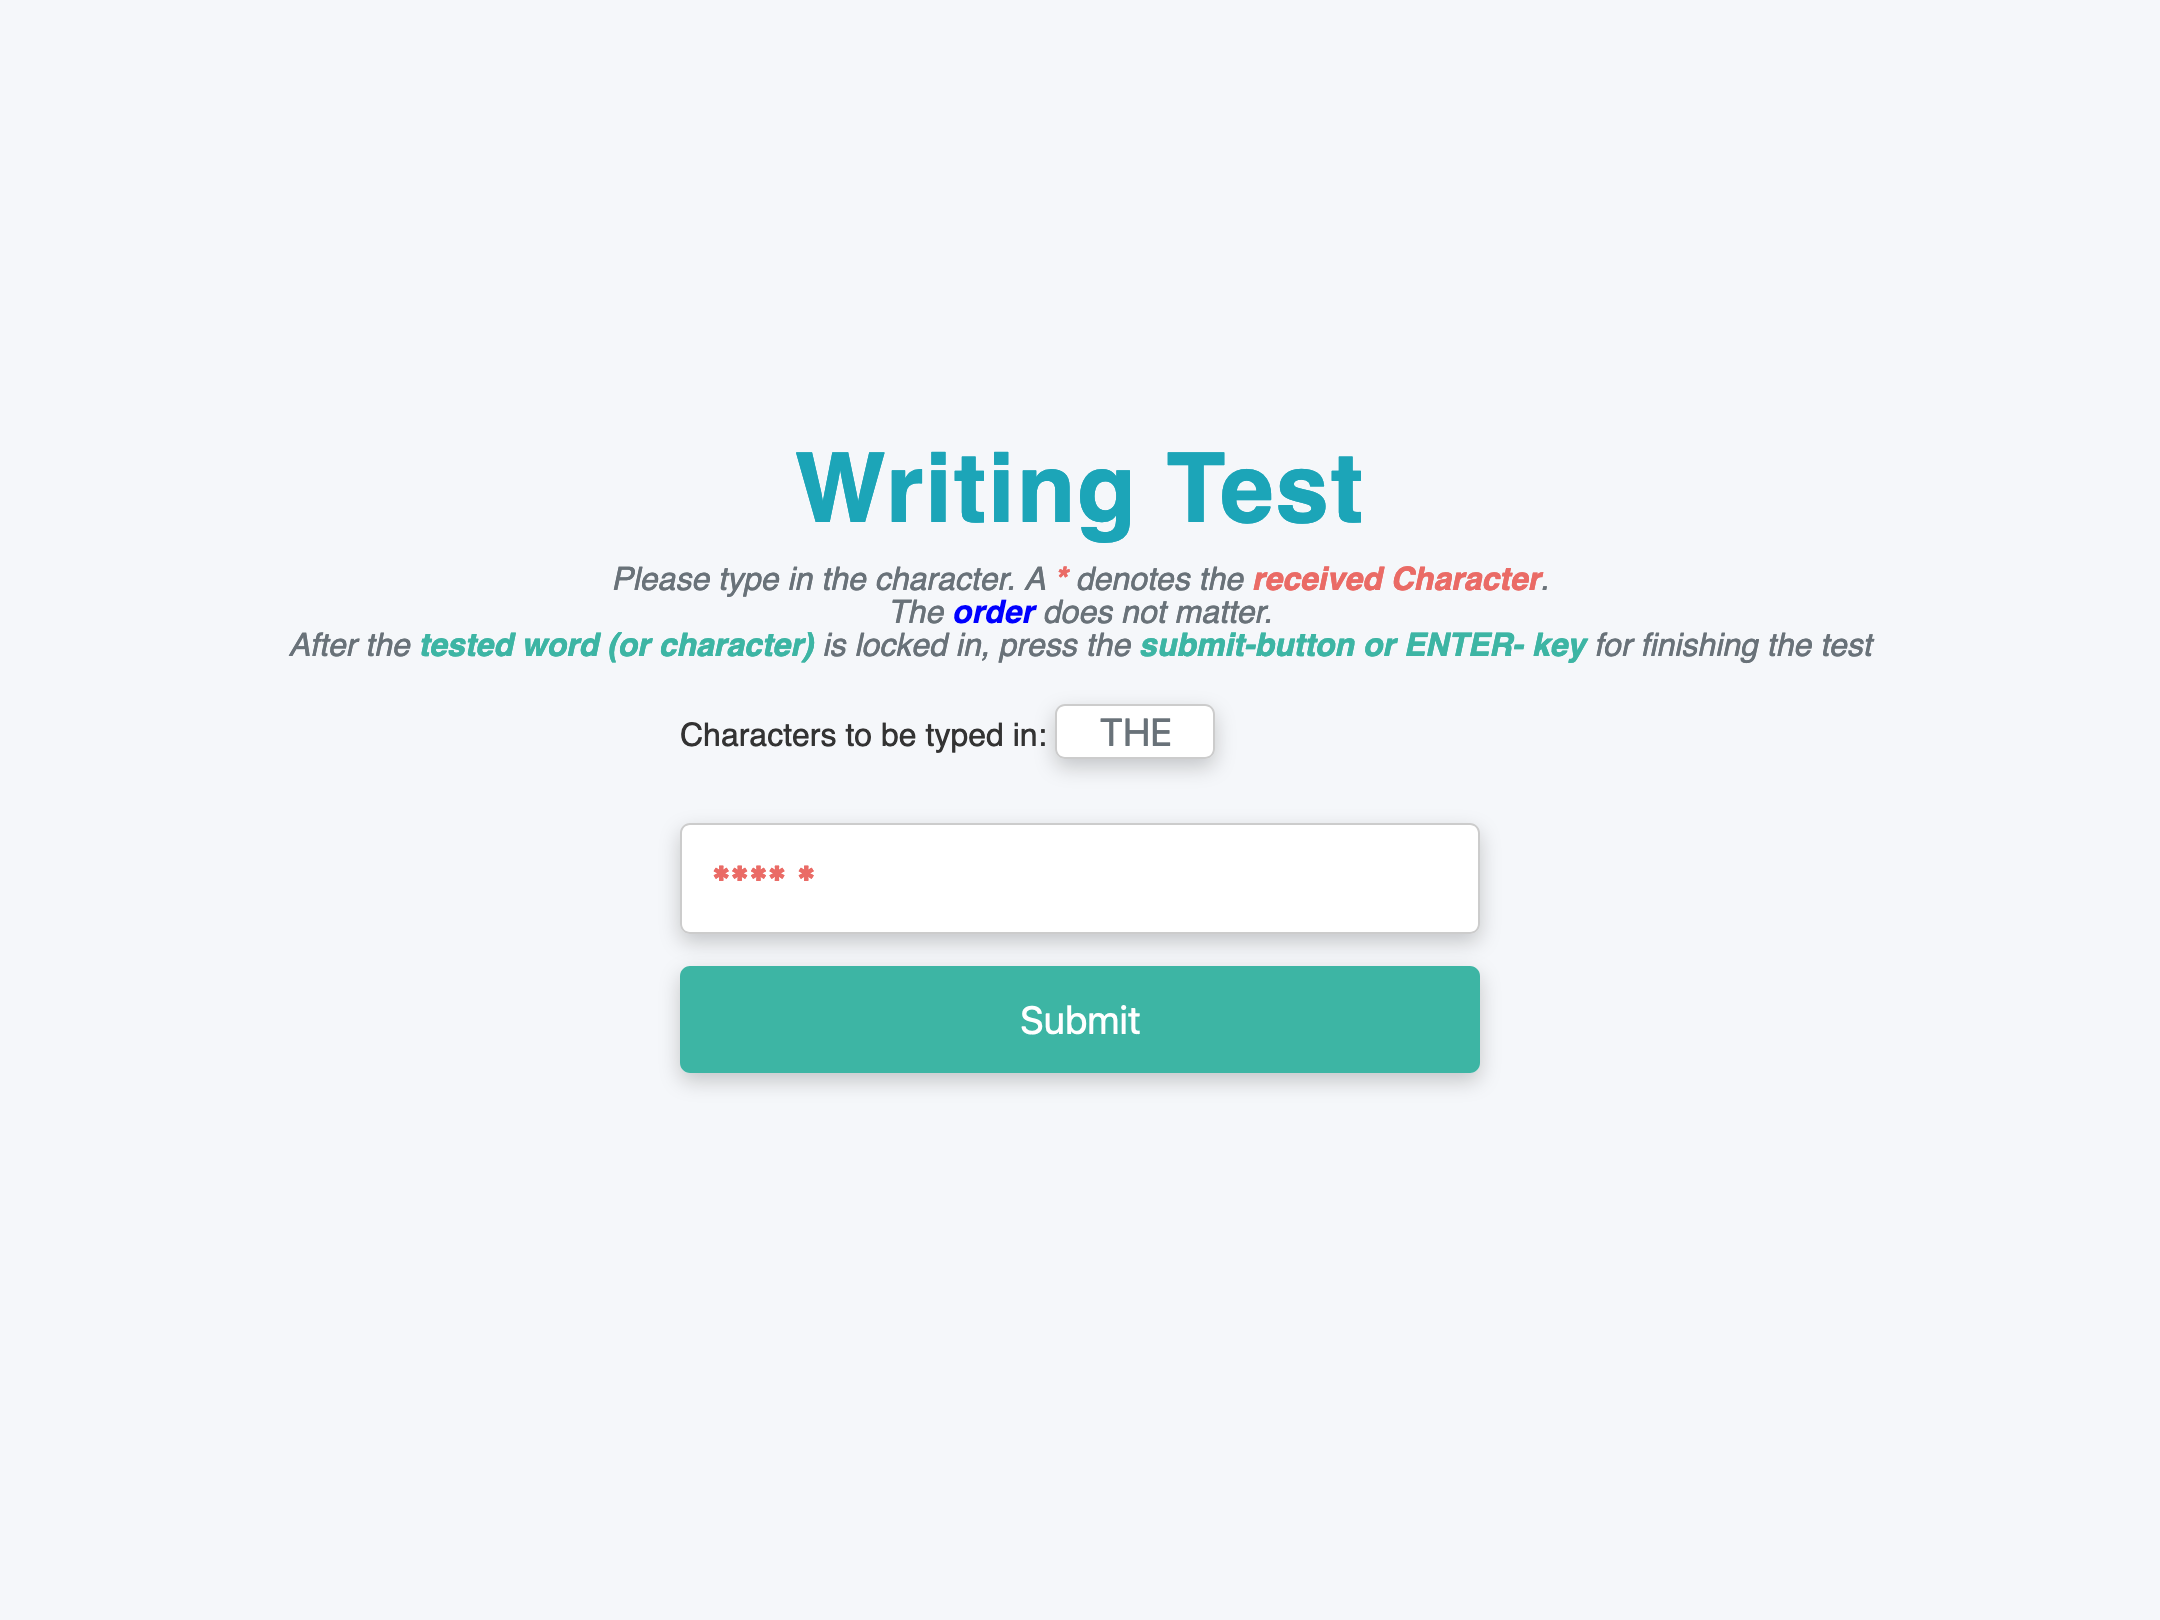
\includegraphics[width=0.5\linewidth]{src/pictures/testingSite.png}
    \caption{Testing Site for the Writing Test.}
    \label{fig:testing-site-Design}
\end{figure}


\subsubsection{Communication between the gloves}
Both gloves operate using a master-slave configuration, with the left glove functioning as the master and the right glove as the slave. To ensure flexibility in actuator motor types and encoding schemes, we implemented a layered architecture within both the master and slave gloves.

For communication, the slave glove employs a listener that, upon receiving a message, triggers a callback function to determine how the data should be processed.

The slave glove can receive two types of data. The first type is the activation sequence, which consists of a series of activation requests and pauses in between. Once this sequence is received, the slave waits for the second type of data—a timing index indicating when the next character should be played.

This approach ensures precise synchronization, as the timing index is transmitted during the pauses between characters, preventing significant timing discrepancies. To meet the requirements of low overhead, fast latency, and high throughput, as outlined in section \ref{Glove_Design_Iteration} 
and illustrated in \autoref{tab:comparissonESPNOW}, we leverage this speed to maintain accurate timing without the need to wait for a connection to be fully established.



\subsection{Encoding Scheme}
This section provides an overview of the encoding methods used in our study. First, we introduce the encoding of chords, which we employ in both of our studies. Here, we differentiate between the sequential approach that we use and the \gls{ost} encoding approach.

The section also discusses the finger activation sequence to ensure alignment with previous works. The second subsection addresses the offset between the audio and the activation sequence that we employ, explaining which method we use and the rationale behind our choice.

The third part focuses on the selection of isograms for the words used during training. We explain why we believe these words to be the most appropriate and demonstrate, using information theory, that they have similar entropy. This selection ensures that the words used for learning are of comparable complexity. Additionally, we explain why our chosen words form a partial pangram.


% We employed two encoding schemes: the \gls{ost} encoding scheme and the spatial-temporal encoding scheme.
% For both schemes, we followed the same finger activation order as Luzhnica et al. \cite{Luzhnica2017}, which demonstrated that activating the fingers in a specific sequence was beneficial.

% The precise timing of these activations is critical to ensure comparability with previous studies.
% The specifications for these timings are detailed in this subsection.

% Additionally, this section explains how we spaced the audio and tactile sensations by comparing our task to similar studies in the field.

% Finally, we discuss the selection of isograms that, together, form part of a pangram.
% We compare these words with those used in previous studies and highlight their shortcomings for our task.
% Specifically, we demonstrate the difference in entropy between the Braille encodings of these words, which provides insight into their effectiveness for our encoding task.


\subsubsection{Encoding Chords}
Encoding Braille words as tactile chords is not straightforward because several considerations must be taken into account, such as how to encode a chord in a way that prevents all fingers from vibrating simultaneously, as this was shown to be ineffective by Seim et al. \cite{Seim2014}, who demonstrated that participants often struggle to distinguish stimuli. Additionally, when offsetting each of the tactile sensations, further considerations must be made, such as: "How long are the sequences activated?" "In which order are the tactile sensations delivered to the fingers?" "How long and where are breaks placed during activation?" and "What activation protocol should we use?" To address these questions, we orient ourselves based on previous works.

For the activation protocol, we use two different encodings, which we compare against each other in the second study. We employ the \gls{ost} encoding developed by Luzhnica et al. \cite{Luzhnica2018, Luzhnica2018a, Luzhnica2017, Luzhnica2016}, as shown in \autoref{fig:chord_encoding}, to encode the chords. The \gls{ost} encoding uses a gap $p$ of 10 ms, following the value named ($g$) used in \cite{Luzhnica2018}, with the same finger stimuli order and tactile thresholds that align with the findings of \cite{Duncan2007}. Additionally, we incorporate the sequential encoding approach used by Seim et al.

The \gls{ost} encoding has several advantages, such as enhanced throughput, as previously outlined. Furthermore, compared to simultaneous encoding, which often leads to difficulties in distinguishing stimuli \cite{Seim2014}, the \gls{ost} encoding has proven more beneficial for learning \cite{Luzhnica2018}. In the first study, we use only the \gls{ost} encoding.

Luzhnica et al. \cite{Luzhnica2017} found that the order in which tactors are activated during overlapping spatiotemporal stimulation impacts the ability to accurately identify stimuli. Prioritizing the activation of tactors, starting with the most sensitive areas, significantly improves accuracy. Building on these findings, we prioritize the fingers according to their known sensitivity order (from index to ring finger), as described by \cite{Luzhnica2017}, \cite{Hoggan2007}, \cite{VegaBermudez2001}, and \cite{Duncan2007}. This prioritization follows the approach outlined by \cite{Luzhnica2017} to enhance perception accuracy.

Studies on temporal acuity indicate that individuals can discriminate between successive taps on the skin with a gap as small as 5 ms \cite{Luzhnica2017, Katz2013}. Luzhnica et al. found that gaps of 10 ms and 20 ms between taps did not significantly impact perception accuracy. Based on this, we chose a gap of 10 ms, as shown in \autoref{fig:audio_vibration_gap}, which is greater than the minimum discriminative gap of 5 ms established by \cite{Luzhnica2017}. This 10 ms gap has been used for \gls{ost} encodings in previous studies \cite{Luzhnica2018, Luzhnica2016}.

During both studies, we use the same intensity for vibration, as \cite{Luzhnica2017} found that varying vibration intensities between tactors does not lead to higher accuracy, even when prioritization by sensitivity is applied. Therefore, we maintain consistent intensities across all tactile sensations.

For the base duration $d$, we use 200 ms, with a between-letter gap (bl) based on the average durations of dots (100 ms) and dashes (300 ms) from \cite{Seim2018} and dots (200 ms) from \cite{Pescara2019}. The 200 ms duration aligns with the recommendations of \cite{Luzhnica2018}, who suggest this interval to separate subsequent letters. While this duration is shorter than those used in some language-teaching studies, such as \cite{Seim2014a}, it fits well within the 100–300 ms range used for keypad learning chords by Seim et al. \cite{Seim2017}.


\begin{figure}
    \centering
    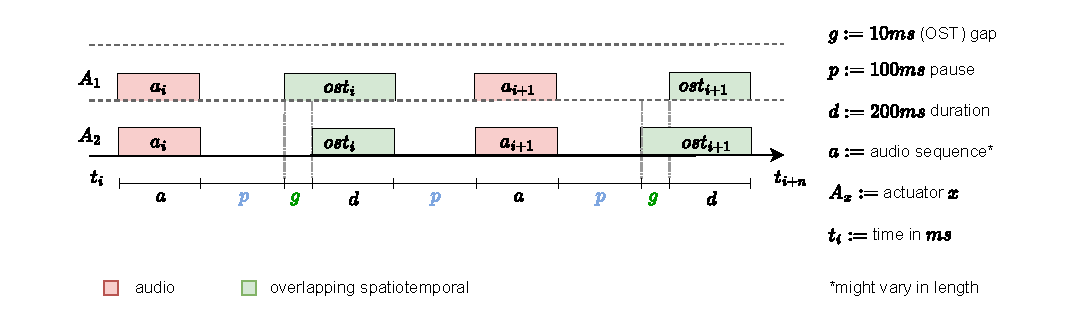
\includegraphics[width=\linewidth]{src/pictures/audio_vibration_diagram.drawio.pdf}
    \caption{Audio vibration offset.}
    \label{fig:audio_vibration_gap}
\end{figure}

\subsubsection{Audio-Chord Offset}
For the offset between audio and vibration, we adopt the same value as used in \cite{Seim2017} for Braille learning, which is 100 ms, as shown in \autoref{fig:audio_vibration_gap}.

For stroking and tapping, we follow the setup described by \cite{Fang2023}, where each finger is stroked or tapped once. However, we use the \gls{ost} encoding with the same \gls{ost} gap and pause time, as illustrated in \autoref{fig:audio_vibration_gap}, so the only difference between the affective and discriminative touch setups lies in the base duration $d$. Since this is the first study, to our knowledge, investigating \gls{ost} with stroking or tapping for affective touch, we use this pattern without any additional prior timing guidelines, except for the passive learning encoding found in Fang et al. \cite{Fang2023}.


\subsubsection{Isogram Selection and carry-over effect minimisation}
\begin{figure}
    \centering
    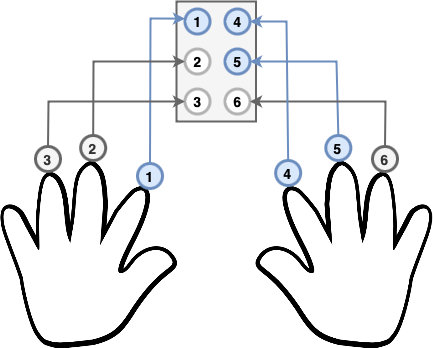
\includegraphics[width=0.5\linewidth]{src/pictures/handBrailleEncoding.drawio.png}
    \caption{Encoding of the character D as an example for hand encodings.}
    \label{fig:hand-encoding}
\end{figure}


When participants are passively learning to type using different actuators, we use a segment of a pangram \cite{Brooke1987}, following the methodology of Seim et al. \cite{Seim2018, Seim2016}. This approach is intended to mitigate the \enquote{carryover effect} \cite{MacFie1989, Brooks2012}, which occurs when participants are influenced by previously learned data, either through stress or prior knowledge.

To ensure a fair comparison and avoid the carryover effect, we taught participants different characters with equal complexity for each actuator. Pescara et al. \cite{Pescara2019} defined complexity by creating patterns of equivalent length and difficulty, based on the number of dash and dot transitions in Morse code. Inspired by this approach, we use entropy, as defined in information theory \cite{Gray2011, Shannon1948, Shannon2001}, to quantify the underlying complexity.

To achieve this, we encoded each Braille dot with a number from 1 to 6, following the methodology of \cite{Yang2017}. The dots correspond to positions on the left hand (index to middle finger) and right hand (index to middle finger), as illustrated in \autoref{fig:hand-encoding} for the Braille character \enquote{D}. Each character is thus represented as a set of numbers corresponding to the Braille dots.

Using this encoding, we calculated the probability \( P(d) \), where \( d \) represents a ``dot at position \( i \).'' We used the standardized English Braille alphabet, consisting of 26 characters. The probability distribution for each dot being present in a character is calculated as:

\[
P(d = X) = \frac{\|\{d \in c \mid c \in A\}\|}{\|A\|}
\]

where \( A \) represents the 26-letter English alphabet. The results are summarized in \autoref{tab:dot-probability}, showing the occurrence of each Braille dot and its corresponding probability across the alphabet.

\begin{table}[!ht]
\centering
\resizebox{.70\columnwidth}{!}{
    \begin{tabular}{c|c|c|c|c|c|c}
        Dot $d$            & \textcircled{1}& \textcircled{2}& \textcircled{3}& \textcircled{4}& \textcircled{5}& \textcircled{6}\\
        Occurrences     & $20$ & $14$ & $15$ & $15$ & $13$ & $6$\\
        $P(d)$     & $0.7692$ & $0.5384$ & $0.5769$ & $0.5769$ & $0.5$ & $0.2307$\\
    \end{tabular}}
    \caption{Probability for each dot occurring.}
    \label{tab:dot-probability}
\end{table}

Using these probabilities for each dot \( P(d) \), we then computed the entropy \( H(c) \) for each character \( c \) using the entropy formula:

\[
H(c) = \sum_{d \in C} P(d) \times \log_2 P(d)
\]

This measures the amount of information in bits per character. The calculated entropies for each character \( c \) are presented in \autoref{tab:entropy-letter}.

\begin{table}
    \centering
    \resizebox{\columnwidth}{!}{
    \begin{tabular}{lccccccccc}
        Character $c$   & \braille{a} A& \braille{b} B& \braille{c} C& \braille{d} D& \braille{e} E& \braille{f} F& \braille{g} G& \braille{h} H& \braille{i} I\\
        $H(c)$ in bits         & $0.2912$ & $0.6458$ & $0.749$ & $1.249$ & $0.7912$ & $1.1036$ & $1.6036$ & $1.1458$ & $0.8124$\\\hline
        Character $c$   & \braille{j} J& \braille{k} K& \braille{l} L& \braille{m} M& \braille{n} N& \braille{o} O& \braille{p} P& \braille{q} Q& \braille{r} R\\
        $H(c)$ in bits         & $1.3124$ & $0.749$ & $1.1036$ & $1.2068$ & $1.7068$ & $1.249$ & $1.5614$ & $2.0614$ & $1.6036$\\\hline
        Character $c$   & \braille{s} S& \braille{t} T& \braille{u} U& \braille{v} V& \braille{w} W& \braille{x} X& \braille{y} Y& \braille{z} Z& ~\\
        $H(c)$ in bits         & $1.2703$ & $1.7703$ & $1.2372$ & $1.5918$ & $1.8006$ & $1.695$ & $2.195$ & $1.7372$ & ~\\
    \end{tabular}}
    \caption{Entropy for each Braille letter rounded to $4$ decimal places.}
    \label{tab:entropy-letter}
\end{table}

We evaluated words used in previous studies, such as ``add,'' ``a,'' and ``bag'' from Seim et al. \cite{Seim2014a, Seim2014}, with entropy values of \( 2.7891 \), \( 0.2912 \), and \( 2.793 \) bits, respectively, and the words ``The,'' ``Lazy,'' and ``Dog''  from Seim et al. \cite{Seim2018}, with entropy values of \( 3.9597 \), \( 5.4531 \), and \( 4.2278 \) bits, respectively.

Next, we searched for a partial pangram composed of three words for the three actuators by going through the English dictionary with word-length of  3\footnote{\url{https://www.dictionary.com/e/word-finder/3-letter-words/}}, while ensuring that the words did not share the same characters and had similar complexity and character length, and are commonly used\footnote{As we didn't interview native speakers we needed to ensure they knew the words}. 
We selected the words ``the,'' ``old,'' and ``pub,'' as shown in \autoref{fig:braille_prestudy_characters}, with entropy values of \( 3.9597 \), \( 3.728 \), and \( 3.6969 \) bits, respectively. These words were deemed more suitable for our task due to their similar entropy values and simplicity, as many of our participants are non-native English speakers. These words were used in the first and second studies (for the second study, we used ``old'' and ``pub'' due to their closer similarity in entropy).

\begin{figure}
    \centering
    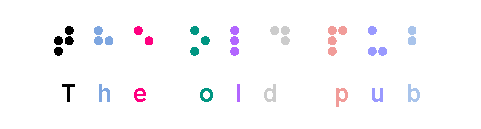
\includegraphics[width=.75\linewidth]{src/pictures/braille_prestudy_characters.drawio.pdf}
    \caption{Sentence used in the pre-study and its braille part.}
    \label{fig:braille_prestudy_characters}
\end{figure}
 











 \section{Study design}

\begin{figure}
    \centering
    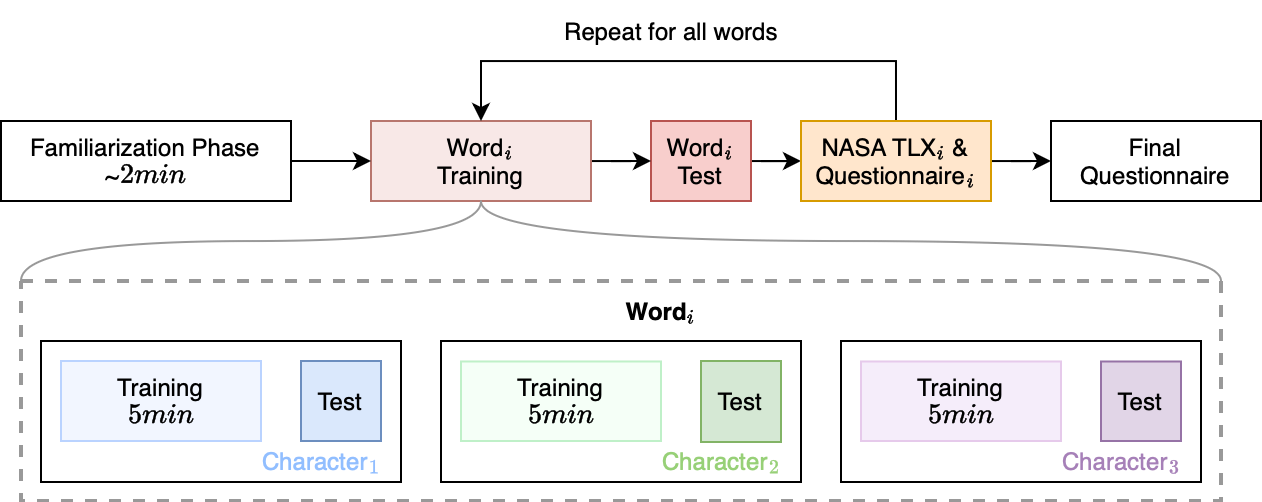
\includegraphics[width=0.75\linewidth]{src/pictures/StudyData/Study_design.drawio.png}
    \caption{Study design.}
    \label{fig:study-design}
\end{figure}

Our study is inspired by the work of Pescara et al. \cite{Pescara2019} and Fang et al. \cite{Fang2023}, and it is divided into two distinct phases. The first phase addresses our first research question: "RQ1: Is there a difference between affective and discriminative touch for both hands using the OST?" This phase is followed by a pre-study. The second phase aims to answer our second research question: "RQ2: Is there a significant difference between using the OST and the SEQ encoding?" In both studies, we focus on teaching uncontracted, alphabetic English Braille, known as Grade One Braille \cite{Troughton1992, Alnfiai2017}.

Similar to Seim et al. \cite{Seim2016, Seim2018}, our studies focus on learning words. However, we use a different set of words than those employed in their research. In the first study, we aim to assess the effectiveness of various stimuli and examine the impact of affective versus discriminative touch using the \gls{ost} encoding. This will be combined with different stimuli to teach Grade One Braille. In the second study, we investigate the differences between using the \gls{ost} and \gls{seq} encodings.

For both studies, we employed a balanced randomized Latin square design, similar to the method used by Huang et al. \cite{Huang2010}, a technique frequently applied in educational and psychological research \cite{Richardson2018}. The study procedures are illustrated in \autoref{fig:study-design}. As shown in the figure, each study begins with a familiarization phase lasting approximately 2 minutes. This phase includes using the testing website \autoref{fig:testing-site-Design} and its input method to familiarize participants with the setup, followed by a brief session of the game Gwelled to help participants acclimate to the game.

The familiarization phase is followed by word training, during which participants use the specific actuator attached to their fingers. For this, we used a Velcro band, similar to the setup used in previous studies \cite{Vaio6810, Fang2023}, enabling comparability with \cite{Fang2023}, which also investigated discriminative and affective touch. For the first study, we used the respective actuator according to the balanced Latin square design, consisting of vibration, tapping, and stroking, with the \gls{ost} encoding employed. In the second study, we used only the vibration actuator, but the encoding was changed according to the balanced Latin square design to either \gls{seq} or \gls{ost}.

During word training, each word is taught letter by letter. The training phase for each letter is followed by a test. In the letter training phase, participants play Gwelled, which was used in previous studies by Fang et al. \cite{Fang2023}, Donchev et al. \cite{Donchev2021}, and Pescara et al. \cite{Pescara2019} for 5 minutes. This serves as a distraction task while they receive their respective stimuli. Throughout this phase, we log user inputs, clicks, game scores, and the time played. This data allows us to assess participant focus in relation to the type of actuator used and evaluate the test results.

To ensure data validity, we monitored the average click count to avoid significant drops between letters with the same stimulus. For the character test, we use the testing site shown in \autoref{fig:testing-site-Design}.

After participants learn three characters, they complete a word test consisting of a word formed from the three learned characters. The word test is conducted on the same website.

During the testing phase, participants do not see their typed information to minimize distractions and encourage better performance, as detailed in \autoref{sub:website}. For each test, participants are given three attempts to reproduce the Braille character chord, following the setup used in previous works \cite{Fang2023, Seim2015, Fang2023a}. After all three characters of a word (as shown in \autoref{fig:braille_prestudy_characters}) have been learned, participants complete a NASA TLX \cite{hart1988development} questionnaire, as well as our own questionnaire assessing the perceived usefulness of the system. Once all conditions (each actuator for the first study or each encoding for the second) are completed, participants fill out a final questionnaire directly comparing the conditions to each other. This final questionnaire aims to gather objective scores for the conditions and determine participants' preferences and feedback. The questionnaires are provided in the appendix.

Since we only have two conditions for the second study, we used only the two Braille words \braille{old} (OLD) and \braille{pub} (PUB), as depicted in \autoref{fig:braille_prestudy_characters}, for learning/testing.
